\documentclass[10pt,a4paper]{article}

% Import packages
\usepackage[utf8]{inputenc}
\usepackage{amsmath}
\usepackage{amsfonts}
\usepackage{amssymb}
\usepackage{xcolor}
\usepackage{caption}
\usepackage[compact]{titlesec}
% Decrease font of subsections
\titleformat{\section}
  {\normalfont\fontsize{12}{15}\bfseries}{\thesection}{1em}{}
\titleformat{\subsection}
  {\normalfont\fontsize{10}{10}\bfseries}{\thesubsection}{1em}{}
\titlespacing\subsection{0pt}{12pt plus 4pt minus 2pt}{0pt plus 2pt minus 2pt}
  
\usepackage{float}
\usepackage{algorithm2e}
\usepackage{graphicx}
\usepackage[left=2cm,right=2cm,top=2cm,bottom=2cm]{geometry}

% Inhoud van titelpagina
\author{Quinten Bruynseraede  \\ R0674455 \and Louis Van Looy \\ R0861408}
\title{The Ethereum network: a graph analysis}

% Kolomlayout
\usepackage{multicol}
\setlength{\columnsep}{1cm}

% Kleine hack om Figures te gebruiken in multicols
\newenvironment{Figure}
  {\par\medskip\noindent\minipage{\linewidth}}
  {\endminipage\par\medskip}

% Gebruik \todo{x} voor rode tekst
\newcommand{\todo}[1]{\textcolor{red}{#1}}
\begin{document}

% Voeg title en authors vanboven in
\maketitle

% Abstract 
\begin{abstract}
	
This work investigates the Ethereum network and more particulary focusses on the transactions of Ethereum. Various graph analysis tools are used to obtain insights about this network. First of all, a descriptive graph analysis of the network is performed, followed by an analysis of the major players in network (called \textit {whale}) to address their role and influence within the network and in the end the community structure of the network is addressed. Six different snapshots are taken of the network, starting in January 2017 and ending in March 2021. 

\end{abstract}

\begin{multicols}{2}

% Nieuwe sectie met \section
\section{Introduction}
The Ethereum network is a blockchain-based network for distributed processing. It contains a thriving ecosystem of distributed applications (dapps), ranging from financial tools to games and gambling. Ethereum's native token is called Ether (ETH), and it has become a acknowledged way of storing and transferring money: a so-called \textit{store-of-value}. In this report, we analyze how ETH is distributed among users, and how it flows between them. In particular, we analyze the role of a group of very wealthy users (called \textit{whales}), and we investigate how important these whales are for the network, and to what degree they contribute to wealth inequality.

In Chapter 2, we introduce some basic concepts related to the Ethereum network. Chapter 3 outlines past work about network analysis of cryptocurrency networks, in particular the Ethereum network. In Chapter 4, we describe how we collected the necessary data. Chapter 6 analyzes the network using a set of network analysis tools, and try to show the importance of whales. Chapter 7 focuses on inequality within the Ethereum network. In Chapter 8, we try to analyze clusters in the network, and try to link these clusters to their utility in the network. 

\section{Ethereum}
% Subsections

In the following section, some fundamental concepts and definitions needed to understand the Ethereum network are explained. Based on this, it is also intended to better understand the network and thus observe and understand the obtained characteristics and network statistics of the network. 

\subsection{Ethereum}
First of all, a formal definition of Ethereum is needed. Ethereum is an open-source, blockchain-based and decentralized software platform. It makes use of its own cryptocurrency, called Ether. The main novelty of Ethereum is its ability to execute smart contracts and create decentralized, distributed applications without any downtime, fraud, control or involvement from a third party. A smart contract can be seen as a piece of code that describes the rules for a transaction between two parties, similar to a written contract. Smart contracts on the Ethereum network are Turing-complete (i.e. they can describe arbitrary computations), and are mostly programmed in the Solidity programming language. 
\subsection{Addresses and transactions}
Users store their Ether in an account, uniquely represented by a 20-byte address, such as \texttt{0xed9a430d9a11616eb1cb07ebc28c9e20a03bd486}. Transactions contain (among other fields), a sender, a recipient and a transaction value expressed in \textit{wei}. 1 Ether is equal to 10e\textsuperscript{18} wei. Smart contracts are also identified by a 20-byte address, and executing these smart contracts can be done by sending them a transaction. All transactions are public by default, but there is no direct link between the identify of a user and his address: the vast majority of transactions happen anonymously. However, several services use addresses that are publicly known. For example, Binance, one of the largest cryptocurrency marketplaces, has at least 20 known addresses \footnote{https://etherscan.io/accounts/label/binance}.
\subsection{Whales}
An important element within the composition of the Ethereum network are whales. Ma \footnote{https://academy.binance.com/en/glossary/whale} gives the following definition:“The term \textit {whale} is used to describe an individual or organization that holds a large amount of a particular cryptocurrency.” This amount is not clearly defined, but within the cryptocurrency community a threshold of around 1.000 of a particular cryptocurrency is being seen as the standard. It is clear that this value can fluctuate, based on the underlying value of the cryptocurrency. In the Ethereum network this threshold is set on owners who own 10.000 Ethereum or more, these holders control approximately 70\% of the total supply of the cryptocurrency\footnote {https://coinmarketcap.com/nl/headlines/news/ethereum-eth-whales-hold-68-percent-total-supply/} \footnote {https://blockworks.co/ethereum-whales-gobble-70-of-eth/}. The choice of the name whale is due to the fact that these parts of the network have a lot of market power within the network and are able to push the market up or down. A whale is not especially limited to an individual, this could also refer an institution or organization that holds a significant amount of cryptocurrencies within the network \footnote{https://academy.binance.com/en/glossary/whale}.


\subsection{The network}
The Ethereum network has seen tremendous growth since its inception in 2015, and contains over 350 million transactions at the time of writing. Since June 2020, the number of daily transactions exceeds 1 million \footnote{https://etherscan.io/chart/tx}. Over 100 million addresses have been registered, and over 600 thousand addresses take part in transactions every day \footnote{https://bitinfocharts.com/comparison/ethereum-activeaddresses.html}. This means a full analysis is generally not feasible.

\section{Related Work}
It has to be said: the literature around graph analysis of the Ethereum network is quite young but strongly emerging. Guo et al. (2019) \cite{GUO201958} were one of the first to address the properties of this network. They investigated the ETH network in the initial phase and in a more developed phase. They found out that several transaction features, such as the transaction volume, transaction relation, and component structure of the graph, exhibit the same heavy-tail property which can be approximated statistically by the power law function. Our work gives a more complete overview of the \textit{evolution} of the network, because we analyze it at six stages instead of just two.\\
Chen et al. (2020) \cite{chenEthereum} performed a graph analysis on the Ethereum network. They focus on the characteristics of its users, smart contracts, and the relationships among them to get a deeper understanding of the network. Money transfers, smart contract creations and smart contract invocations are central within their work. These three elements are vital for the users to send money, to create smart contracts on Ethereum, and for the users or applications to invoke the created smart contracts. In this work, metrics like degree distribution, degree centrality, Pearson coefficient, clustering coefficient and PageRank are used and is therefore a good benchmark for this work.\\
Victor \& Lüders (2019) \cite{inbook} focus on the trade of tokens on the Ethereum network, more specifically called ERC20 token networks. These tokens can be seen as digital assets, built on top of ETH and strengthen the Ethereum ecosystem by driving demand for ETH, needed to power the smart contracts. They provide an overview of 64,000 ERC20 token networks and focus graphically on the top 1,000. In this work, they observe that the token networks are frequently dominated by a single hub and spoke pattern, supplemented with very small clustering coefficients. The token network looks disassortative and a lot of the network activity is directed towards exchanges whereby many owners never transfer their tokens at all. As ERC-20 tokens can be considered a smart contract, we will not spend much time investigating this aspect, but they are an indispensable part of the Ethereum ecosystem.


\section{Data collection}
Given the size of the Ethereum network, we have to resort to sampling techniques. One type of sampling uses \textit{random walks}, that start at a given point and follow edges while collecting the necessary data. Random walks are particularly useful for networks where it is not possible to delimit a part of the network in advance \cite{Becchetti06acomparison}. Ethereum is such a network: addresses are not ordered or structured in any way. We collect transactions using a Breadth-first search (BFS). To analyze the evolution of the network, we create six separate snapshots: each snapshot spans 1 month and is limited to 1 million transactions.

\medskip
\begin{algorithm}[H]
\SetAlgoLined
\hspace{5pt}\texttt{T} = $\emptyset$\newline
Initialize \texttt{Queue} with 100 known addresses
\While{\texttt{T.size} $\leq$ 1e6}{
\hspace{5pt}1. Pop an address \texttt{A} from \texttt{Queue}\newline
2. Fetch all transactions by \texttt{A} during the specified time period \newline
3. Add all transactions to \texttt{T} \newline
4. Add all addresses that occur in these transactions to \texttt{Queue }\newline 
} 
\end{algorithm}

Although transactions contain many more features, only the columns \texttt{from}, \texttt{to}, and \texttt{value} are used.
Each snapshot can then be considered a graph: nodes are addresses and edges are transactions between addresses. The value of the transaction is the weight of the edge. If multiple transactions occur between the same pair of addresses, the sum of their according values is taken. 

The following table shows the size of each snapshot:\\
\vspace{5pt}
\bgroup
\def\arraystretch{1.5}
\begin{tabular}{p{0.1\textwidth}|p{0.1\textwidth}|p{0.1\textwidth}|p{0.08\textwidth}}
\textbf{Snapshot} & \textbf{\#txs} & \textbf{\#nodes} & \textbf{\#edges} \\ 
\hline 
Jan '17 & 475 598\footnote{Queue was empty before 1M transactions could be collected.}& 81 242 & 186 942  \\
Nov '17 & 988 086 & 548 355 & 657 697  \\
Sep '18 & 1 000 258 & 528 506 & 635 623 \\
Jul '19 & 1 006 153 & 550 393 & 673 967 \\
May 20 & 1 003 812 & 474 030 & 580 773 \\
Mar '21 & 1 001 864 & 566 733 & 701 482 \\
\end{tabular}
\egroup

To account for seasonal effects, the time between two snapshots is always 10 months. We also don't consider the state of the network before January 2017, when it was still relatively new and the number of transactions was low.

\section{Analysis of the Ethereum network}
In this section, we look at some global characteristics of the Ethereum network. Wherever possible, we show how these characteristics evolved over time.
\subsection{Degree and transaction volume}
First of all, it appears that the average degree of the first snapshot in Jan'17 is high, 4.602, whereas in the following snapshots this number is significantly lower and lies within the range of 2.398 and 2.476. We suspect the smaller size and consequentially larger influence of the starting addresses cause this larger average degree in 2017.

Figure \ref{tbl-degreedistributions} shows the degree distribution for each snapshot. The distribution appears to follow a power law at first (estimated $k^{-2.1}$), but as the degree increases, the distribution is more or less uniform. In particular nodes with a degree above 5000 would be very rare in a perfect scale-free network, but we observe them often. It is noteworthy that Guo et al. \cite{GUO201958} find a power law distribution with an exponent of $k = 3.23$, whereas we find $k=2.1$. We suspect this difference can be explained by our data collection method, which favours nodes with a high degree (i.e. transactions with many other nodes).
\end{multicols}

\begin{figure}[h]
\centering
\begin{minipage}[t]{.33\textwidth}
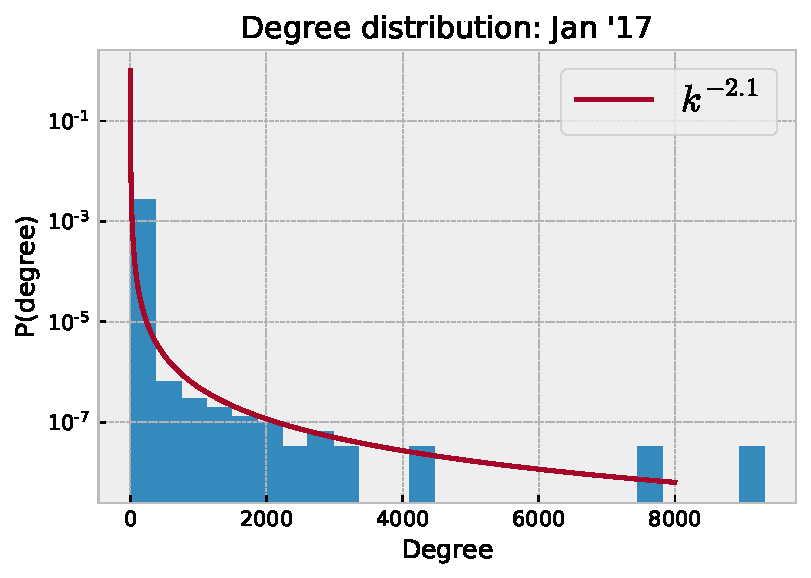
\includegraphics[scale=0.4]{figures/degree_dist_jan_17.pdf}
\end{minipage}%
\begin{minipage}[t]{.33\textwidth}
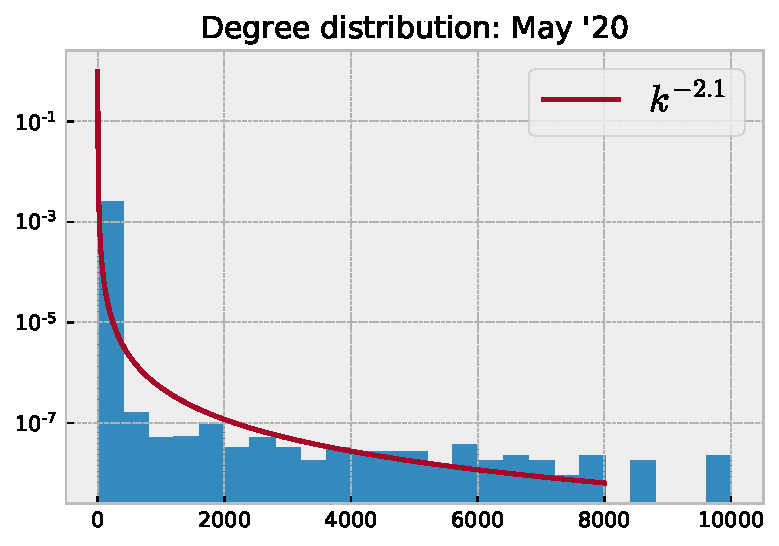
\includegraphics[scale=0.4]{figures/degree_dist_nov_17.pdf}
\end{minipage}
\begin{minipage}[t]{.33\textwidth}
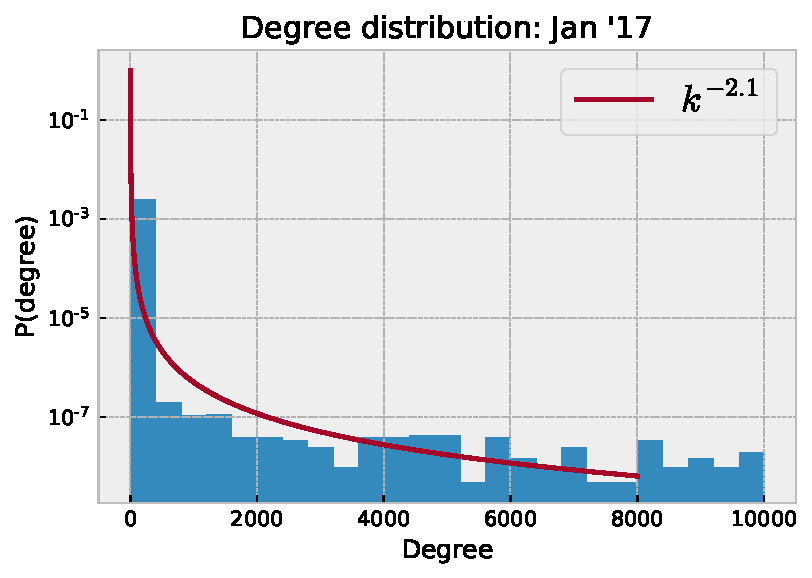
\includegraphics[scale=0.4]{figures/degree_dist_sep_18.pdf}
\end{minipage}\\
\begin{minipage}[t]{.33\textwidth}
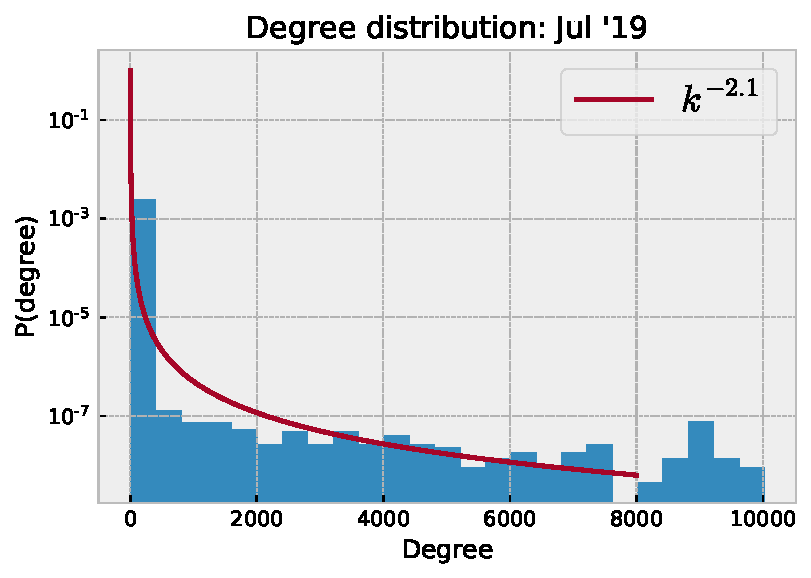
\includegraphics[scale=0.4]{figures/degree_dist_jul_19.pdf}
\end{minipage}%
\begin{minipage}[t]{.33\textwidth}
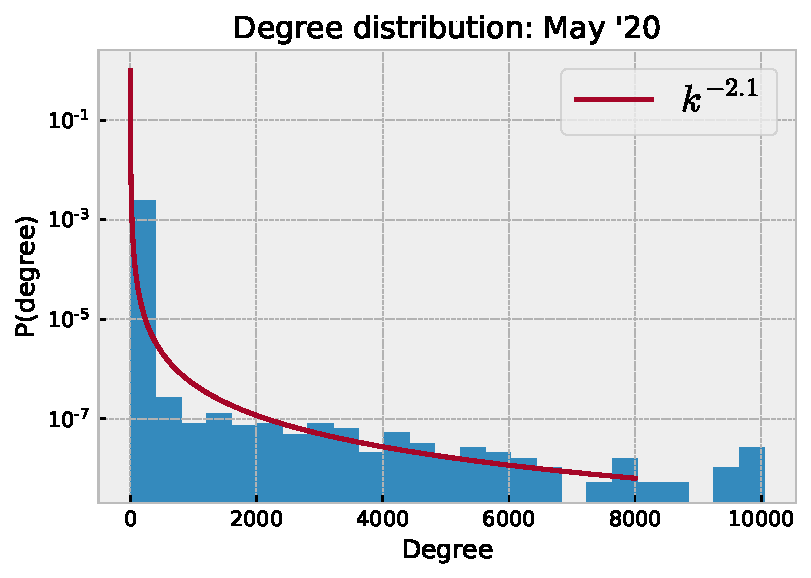
\includegraphics[scale=0.4]{figures/degree_dist_may_20.pdf}
\end{minipage}
\begin{minipage}[t]{.33\textwidth}
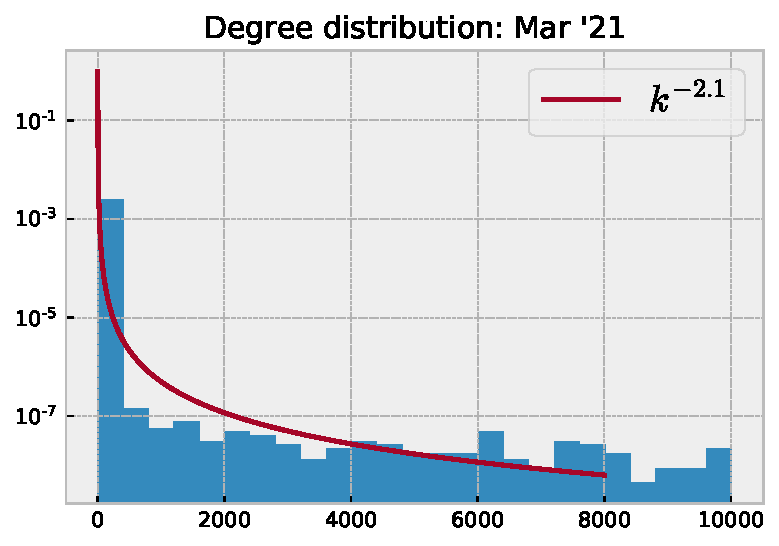
\includegraphics[scale=0.4]{figures/degree_dist_mar_21.pdf}
\end{minipage}%
\caption{Degree distribution for all snapshots}
\label{tbl-degreedistributions}
\end{figure}

\begin{multicols}{2}
Next, we look at the transaction volume in each snapshot. For our network, the transaction volume of a node is simply the sum of all outgoing transactions. Similar to what Guo et al. discovered \cite{GUO201958}, the transaction volume appears to follow a power law.

\begin{Figure}
\centering
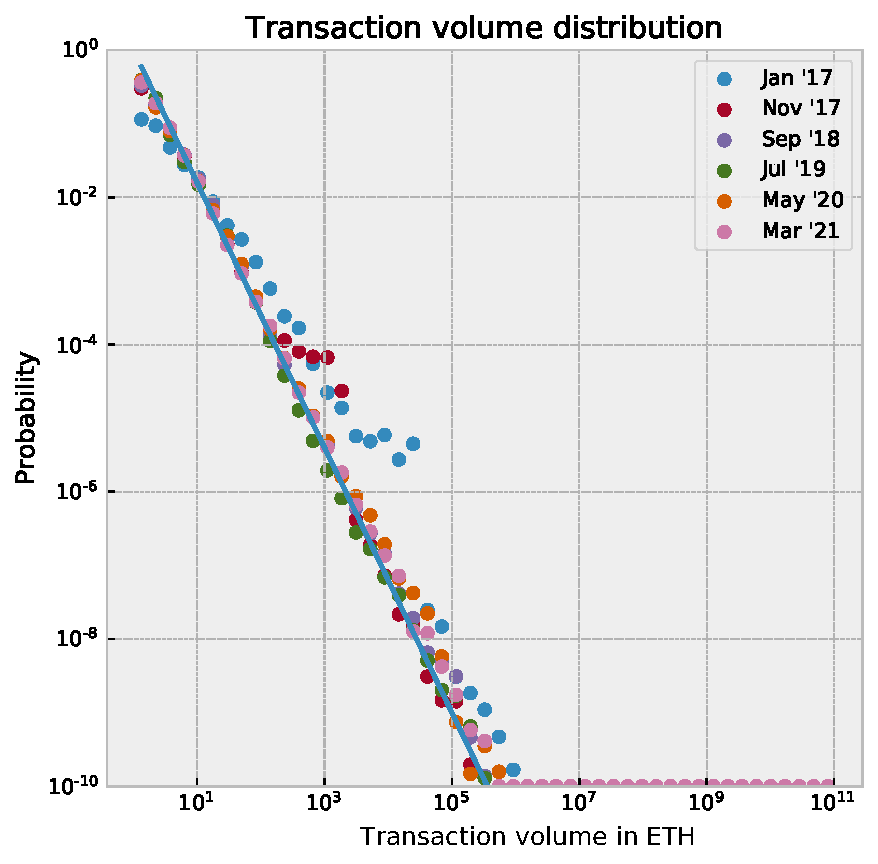
\includegraphics[scale=0.53]{figures/transaction_volume.pdf}
\captionof{figure}{Distribution of transaction volumes}
\end{Figure}

This logarithmic plot shows how the transaction volumes are distributed for each snapshot. First of all, it appears that transaction volumes have not changed much over time. A deviation is observed in the 2017 snapshots, in which transaction volumes were a bit higher than average. We suspect this deviation may be caused by the so-called \textit{2017 bull run}, a period of spiking prices, which attracted many new investors. Interestingly enough, the bull run that is currently ongoing is not reflected in the transaction volumes of the March 2021 snapshot.

\subsection{Small-world characteristics}
Many networks can be considered \textit{small-world networks}: they have a) a high clustering coefficient, and b) a low average path length \cite{WattsDuncanJ1998Cdos} (often $L \propto log(N)$). Compared to random graphs generated with the Erd\"{o}s-R\'{e}nyi model, small-world graphs have many cliques or near-cliques, and many hubs: nodes that connect cliques and facilitate shorter path lengths.

The Ethereum network on the other hand, has a very low clustering coefficient: in all snapshots, we measured this coefficient as less than 1e-4. In their original paper, Watts and Duncan demonstrate small-world networks with clustering coefficients up to 0.79, so the Ethereum network is certainly not heavily clustered. Apart from January 2017, where the clustering coefficient was a bit higher, it has remained more or less constant. 

\begin{Figure}
\centering
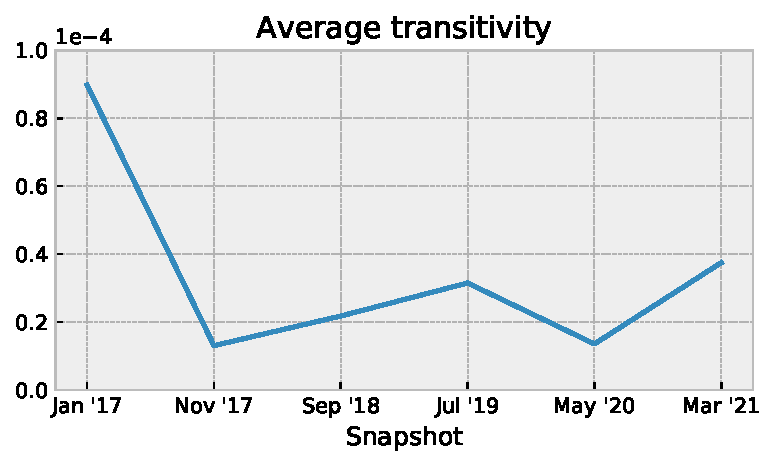
\includegraphics[scale=0.55]{figures/transitivity.pdf}
\captionof{figure}{Evolution of transitivity over time.}
\end{Figure}

The average geodesic path length, however, is very small, and appears to be in the order of magnitude that is required for a small-scale network: $L \propto log(N)$. 

\begin{Figure}
\centering
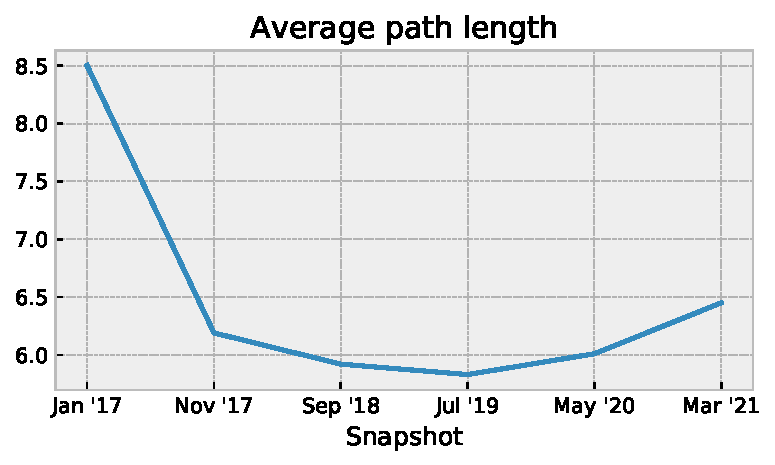
\includegraphics[scale=0.55]{figures/average_path.pdf}
\captionof{figure}{Evolution of transitivity over time.}
\end{Figure}

Remarkably, for both transitivity and average path length, the January 2017 snapshot appears to be an outlier: we suspect that the lower number of nodes leads to a slightly higher average.

Based on these metrics, we can conclude that the Ethereum is not a typical small-world network: the network is not nearly clustered enough. However, the average path length is quite small. We suspect that the network is structured as a number of highly-active hubs (most likely exchanges), that trade with many individual users directly. These users rarely trade among themselves. This claim is also supported by the degree distribution: a very large part of the network has only one connection. Furthermore, many addresses likely belong to individual users, who have no intention of trading regularly, but just hold Ether as a long-term investment.

\vspace{5pt}
\begin{Figure}
\centering
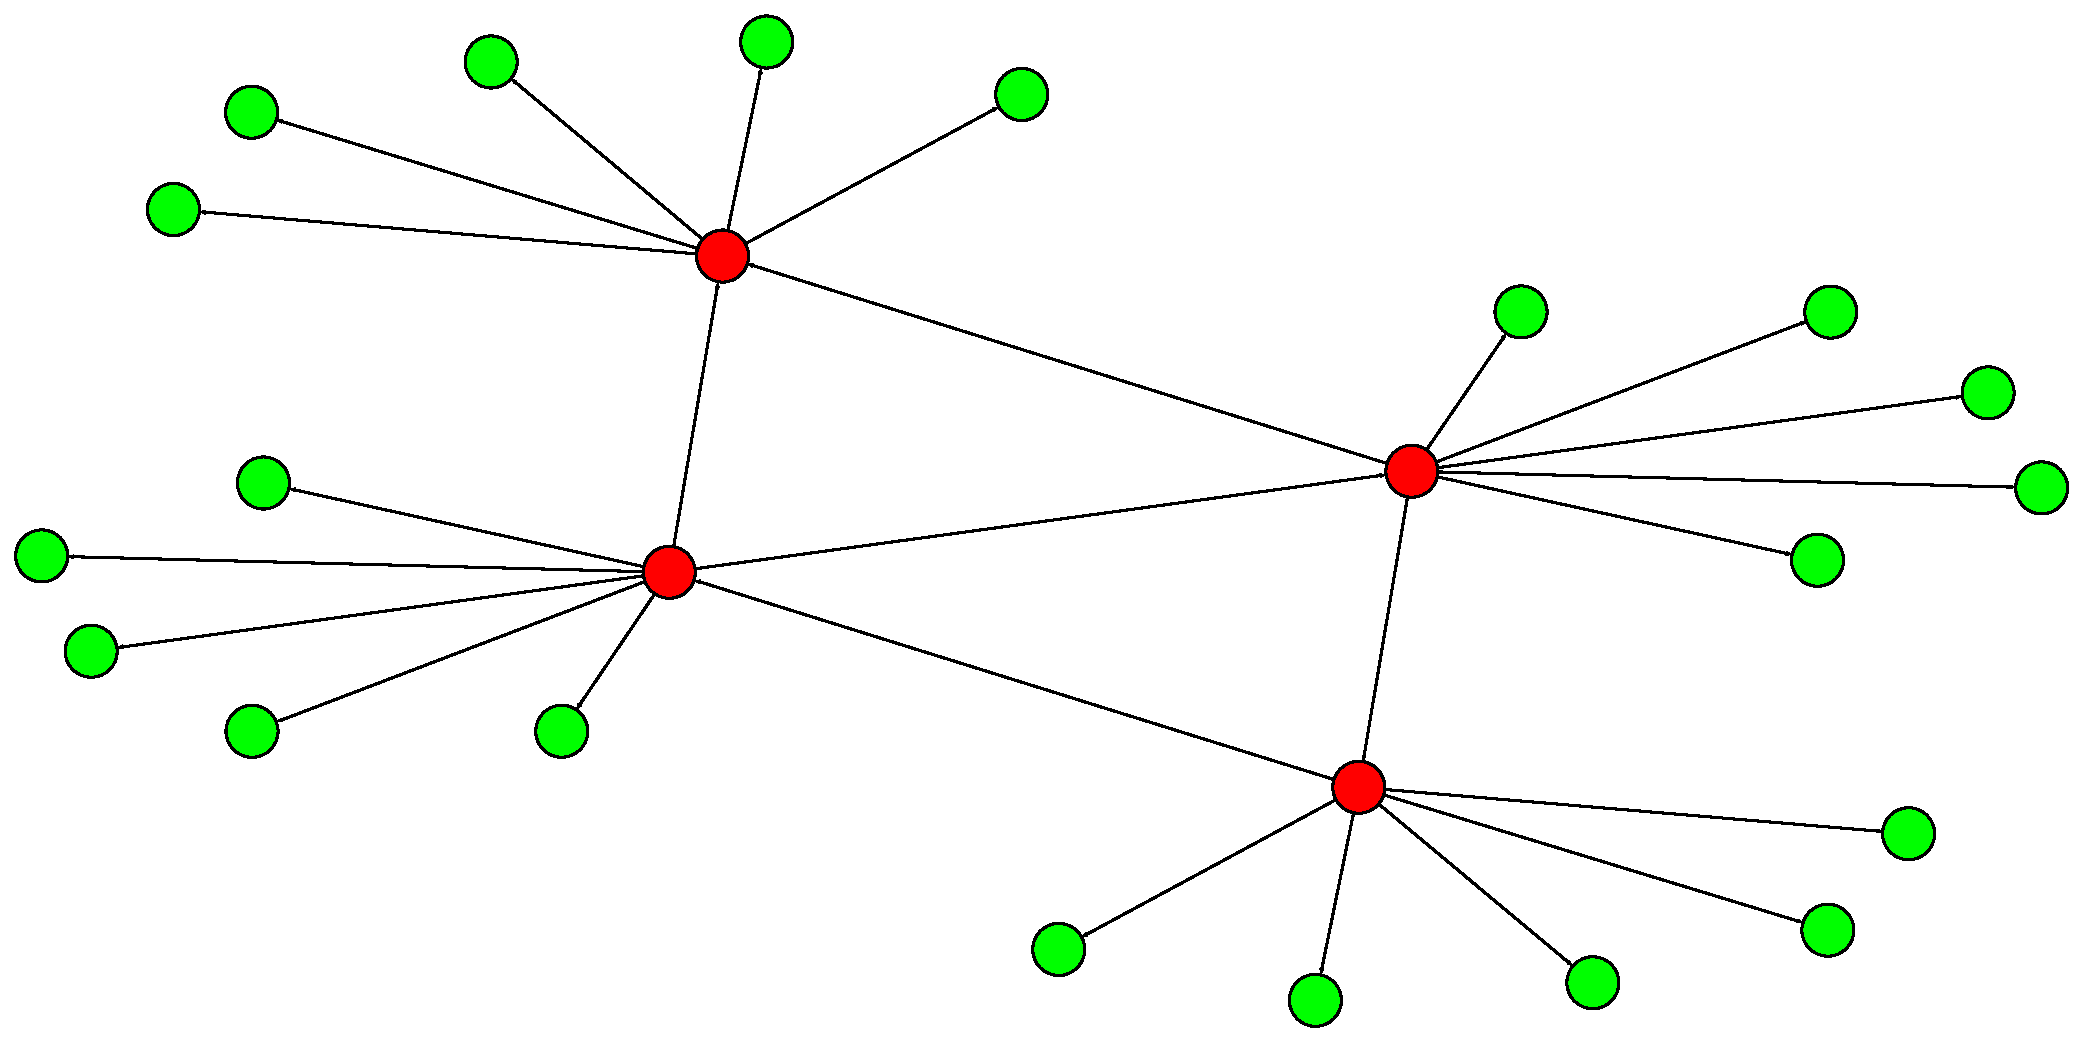
\includegraphics[scale=0.2]{figures/actual_structure.pdf}
\captionof{figure}{Structure of Ethereum network (red nodes are 'hubs', green nodes are 'users').}
\end{Figure}

\subsection{Whales}
We now shift our focus to whales. Here we define those as addresses that posses at least 10 000 ETH. Unfortunately, it is not possible to identify whales in the past: finding out the balance of an address at a certain point in times requires backtracking the entire Ethereum blockchain, which is over 4 terabytes large. Therefore, our analysis of whales is limited to the current situation and how the situation changed over time.

Currently, 1292 addresses are considered whales. Our most recent snapshot (March 2021) includes transactions from more than 500 000 addresses, of which \textbf{60} are whales. Despite making up less than 0.01\% percent of the network, whales account for a trading volume of more than 25\% (2.33 million out of 9.26 million ETH). Obviously, this imbalance can partially be attributed to the fact that whales have the capacity to trade large amounts, but it strengthens our suspicion that whales are very important traders, and may coincide with hubs.\\

We induce a subgraph by selecting all whales and the edges between them. We can now compare the full network with this subgraph.

\vspace{5pt}
\bgroup
\def\arraystretch{1.5}
\begin{tabular}{p{0.2\textwidth}|p{0.12\textwidth}|p{0.07\textwidth}}
 & \textbf{Full graph} & \textbf{Whales} \\ 
\hline 
Shortest path length & 6.46 & 1.84 \\
Transitivity & 3.7e-5 & 0.06\\
Diameter & 22 & 4 \\
\end{tabular}
\egroup
\vspace{5pt}

These differences indicate that whales are somewhat more connected between themselves than the entire network. However, these numbers have to be compared carefully, as there are only 60 whales, which naturally leads to shorter paths and a smaller diameter of the network. Transitivity, however, is a relative metric and shows an increased connectedness between whales. Still, from an absolute point of view, a transitivity of 0.06 is not high: we can definitely not conclude that many whales are directly connected.

Figure 6 shows a visualization of the 60 whales we found in March. Fortunately, some addresses are publicly known and can be linked to their organization or goal. As expected, most whales orginate from cryptocurrency exchanges and a large portion of whales remains anonymous. We also show which whales interact with each other, and the node size is proportional to the addresses' balance in March 2021. 

\vspace{5pt}
\begin{Figure}
\centering
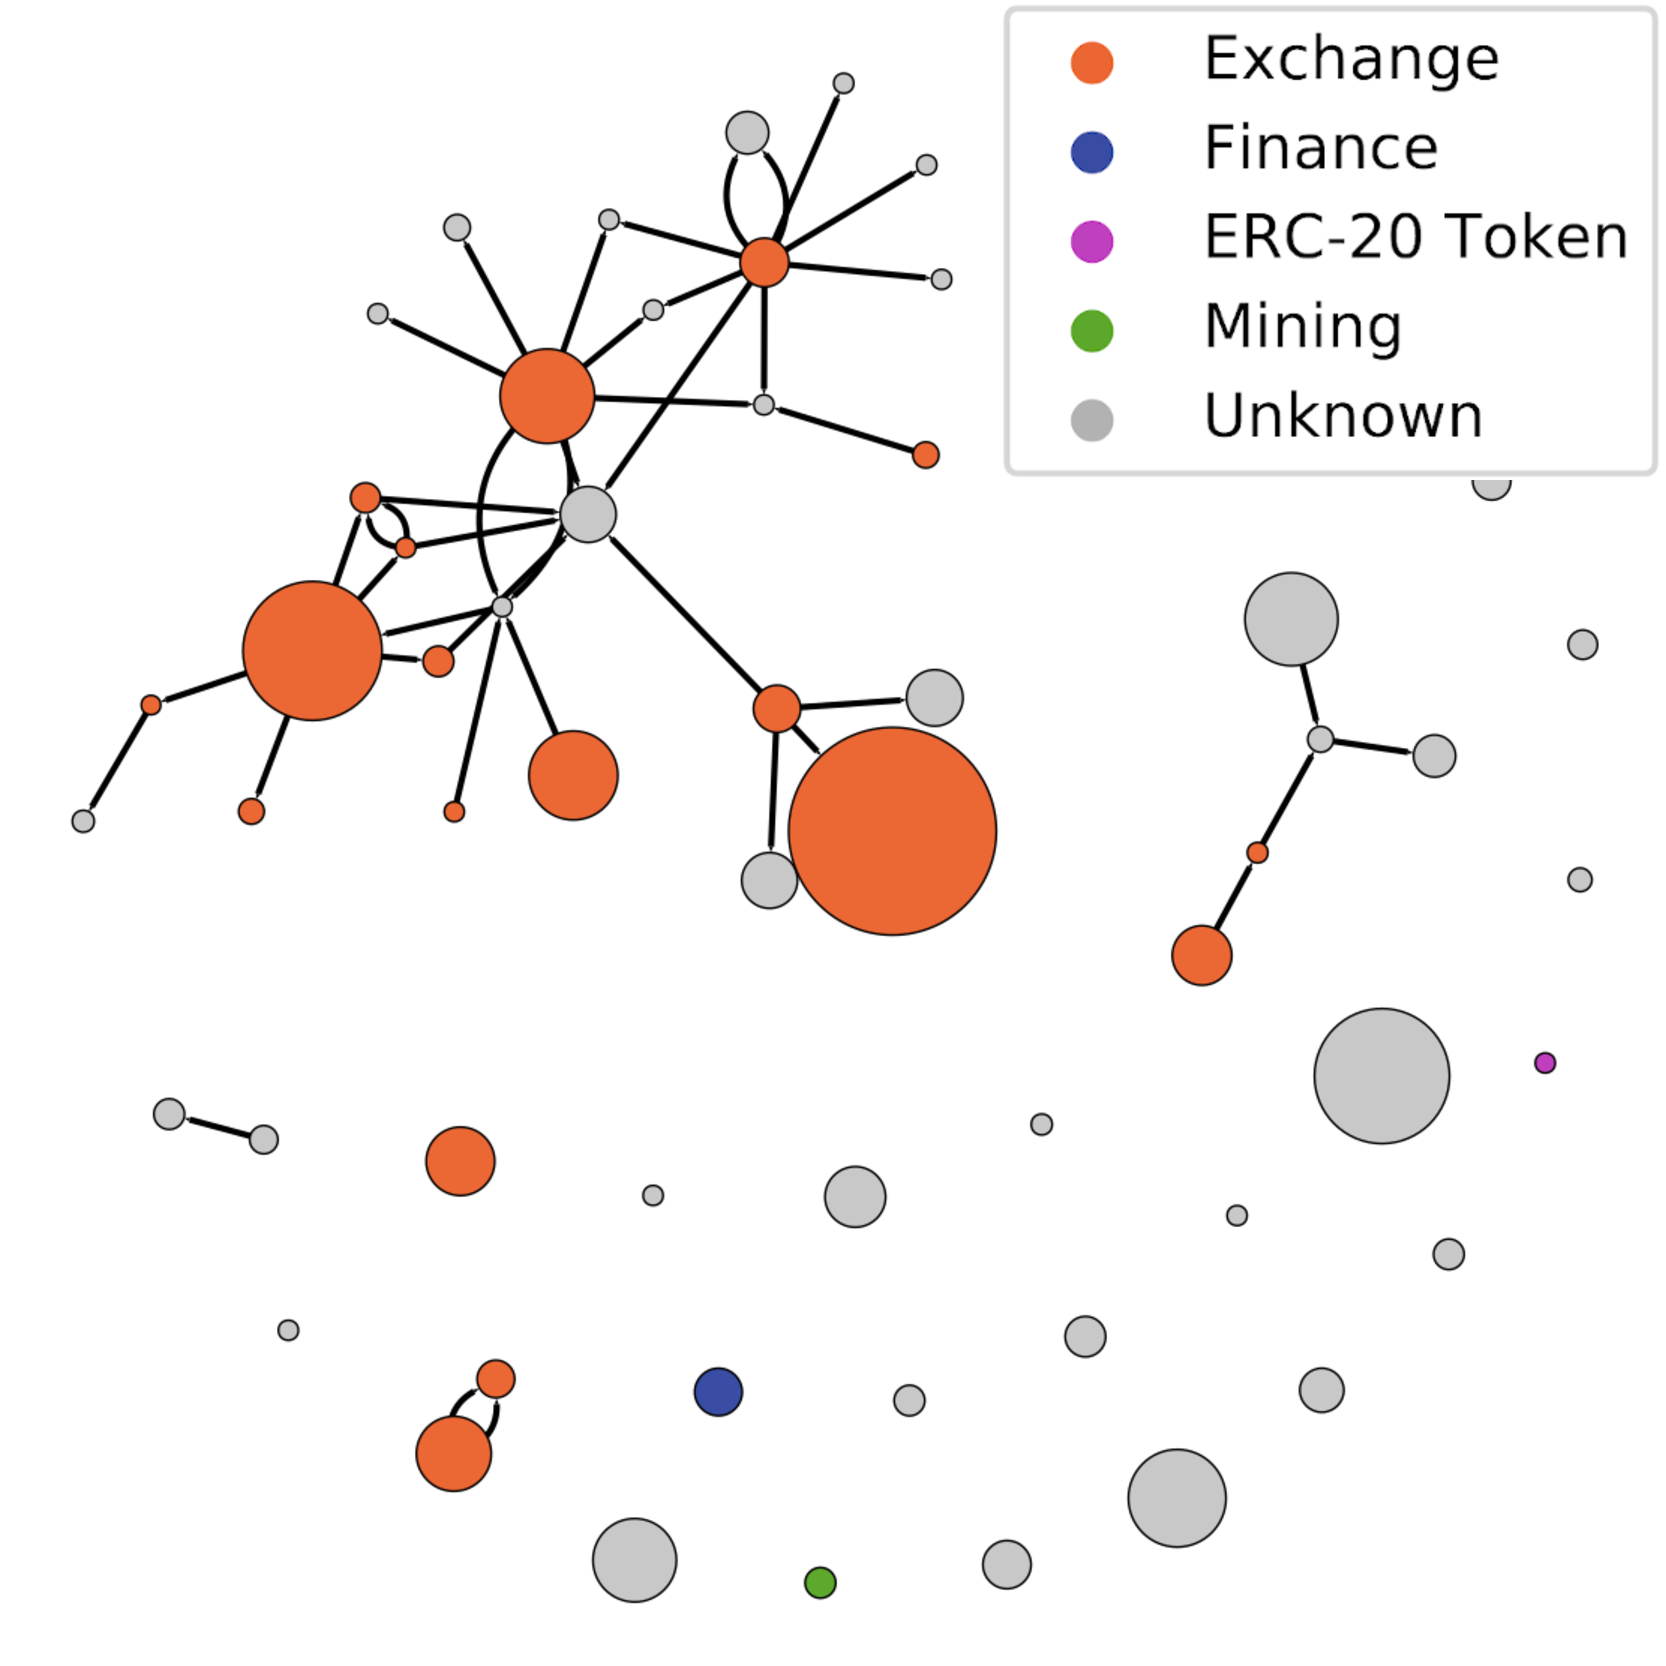
\includegraphics[scale=0.23]{figures/whales.pdf}
\label{whales}
\captionof{figure}{Visualization of whales by address type.}
\end{Figure}

We conclude:
\begin{itemize}
\item{Almost all whales are exchanges.}
\item{All exchanges trade with other whales.}
\item{Non-exchange whales do not trade as much with other whales.}
\end{itemize}

As we expected, exchanges form an important and highly connected backbone to the network. They hold and trade large amounts of Ether. Other applications that make use of the Ethereum network (such as mining, financial products and tokens) do not play such a large role yet. This also confirms our suspicion that Ether is nowadays mostly traded as an investment; we do not yet observe a large amount of activity between users and applications on the Ethereum network.

\section{Community detection}
Previously, we investigated cluster-like structures among whales. We now apply proper community detection techniques to each snapshot, using the modularity measure to evaluate the clustering. Given the size of our networks, an efficient technique is desired. Additionally, we have no prior expectation about the number of clusters in our network. The following clustering approaches have been analyzed: 
\begin{enumerate}
\item{\textbf{Louvain method:} a divisive method that claims linear time complexity on sparse graphs. Its hierarchical nature may also help resolve the resolution limit problem \cite{Blondel_2008}.}
\item{\textbf{Leiden method:} an improvement to the Louvain algorithm that prevents communities that are badly connected or even completely disconnected \cite{leiden}.}
\item{\textbf{Eigenvector method:} this method expresses modularity in terms of eigenvectors of the so-called \textit{modularity matrix} \cite{Newman_2006}. The recursive implementation of this method will keep splitting communities until no longer possible, or a fixed number of communities is reached. To prevent it from endlessly splitting, we set the maximum number to 100, a bit higher than the average number of clusters by the Leiden and Louvain methods.}
\end{enumerate}

Figure \ref{clusters} shows the results of community detection.
\vspace{5pt}
\begin{Figure}
\centering
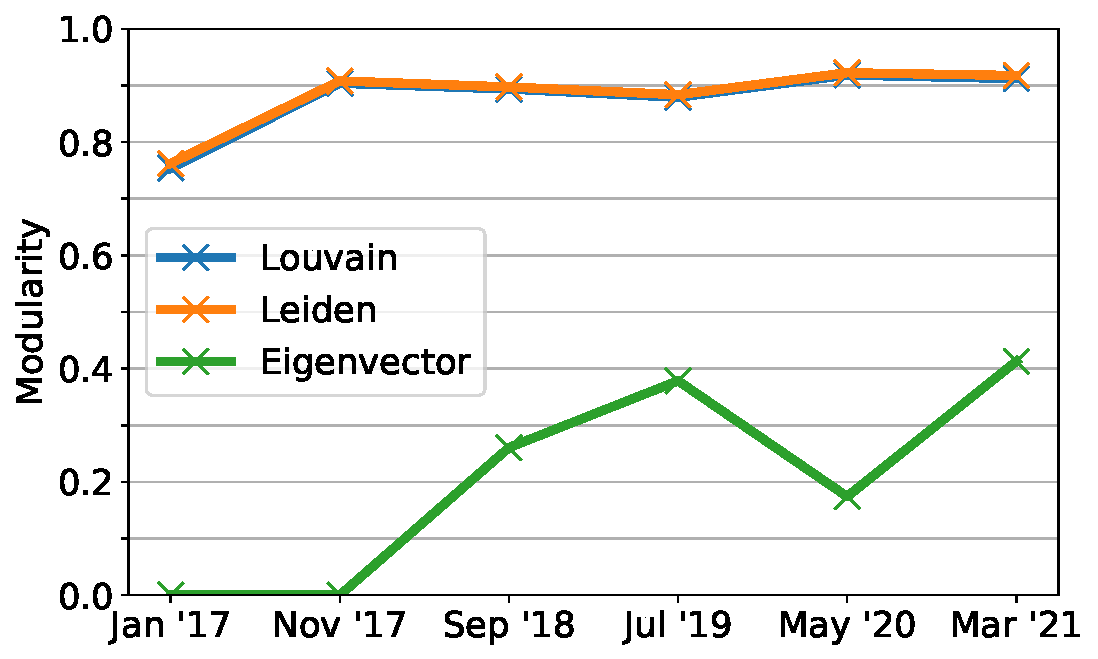
\includegraphics[scale=0.45]{figures/clusters_modularity.pdf}
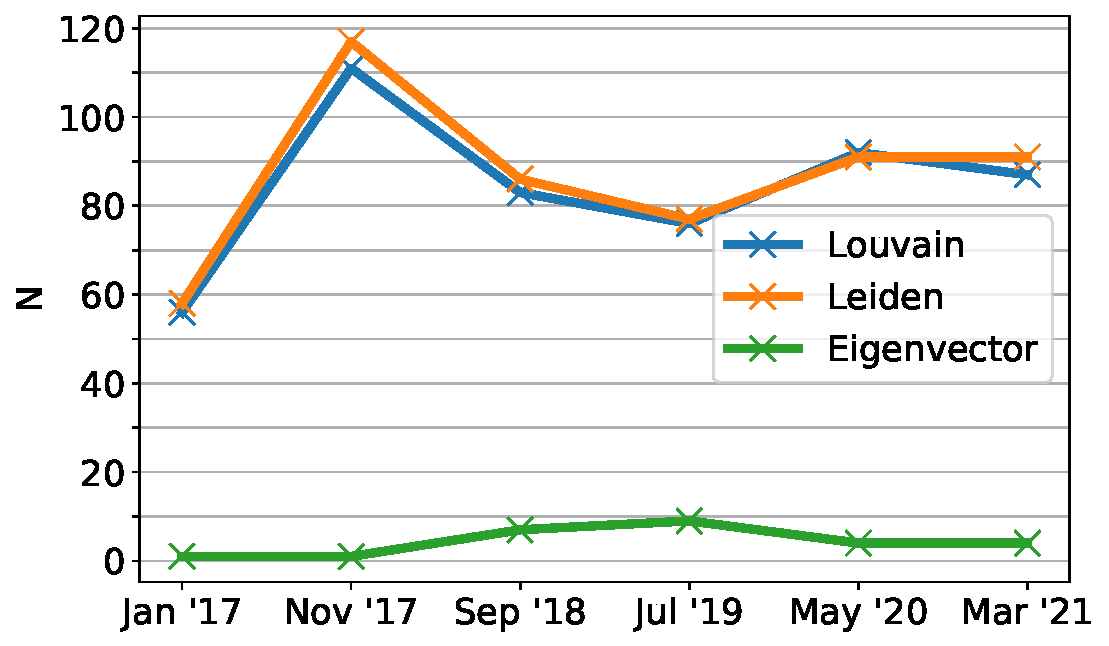
\includegraphics[scale=0.45]{figures/clusters_num.pdf}
\label{clusters}
\captionof{figure}{Modularity and number of clusters for three clustering methods.}
\end{Figure}

Clearly, the Louvain and Leiden methods find very similar clusterings. This leads us to believe that the principal problem that Leiden tries to overcome (badly connected communities), does not occur in our networks. The modularity of their clusterings is very high (The number of communities is quite stable over time between 70 and 90. Again, we observe a deviation in the first snapshot, caused by the smaller network size. 

The eigenvector method yields very different result: a low number of clusters (often even 0) and a modularity under 0.4.

\end{multicols}
\bibliographystyle{plain}
\bibliography{references}
\end{document}
